\documentclass[11pt]{article}
\usepackage[margin=0.9in]{geometry}
\usepackage{fontspec}
\setmainfont{Helvetica Neue}
\usepackage{graphicx,booktabs,enumitem,float,array,caption}
\usepackage{xcolor}
\usepackage[colorlinks=true,urlcolor=blue!60!black,linkcolor=black]{hyperref}
\setlist{nosep,leftmargin=1.3em}
\setlength{\parindent}{0pt}\setlength{\parskip}{5pt}
\title{n-shot Style Prompting of Orpheus Hindi (Pretrained)\\with Natural MaSaC Speech}
\author{cs-tts-steering project}
\date{November 12, 2026}
\begin{document}
\maketitle

\section*{Headline Findings}
\begin{itemize}
\item \textbf{Natural speech in the prompt makes the model unstable.} With natural shots, the model often never emits end-of-speech and runs until the token cap: 13/30 clips at 1 shot, 23/30 at 3 shots, 19/30 at 5 shots. With no shots it happens in 1/30, and with its own synthetic shots in 3/30 (Figure~2). This one failure drives most of the averages below: longer clips, higher CER, lower mean speaker similarity.
\item \textbf{The voice can be cloned, but not reliably.} Many natural-shot clips reach a speaker similarity of 0.90--0.97 to the target speaker, at the level of the speaker's own recordings. Others collapse to 0.2--0.4, almost all of them runaway clips (Figure~3). This is clearest for Maya: the model's default voice is far from hers (0.79), and the clean clips move close to her.
\item \textbf{Prosody moves partly toward natural speech, and only with natural shots.} Pitch variability (F0 SD, F0 range) rises from about 2.9 semitones with no shots to 3.5--4.2 with natural shots. Natural speech is at 5--7, and the model's own shots lower it (2.2--2.6). The rise is consistent in direction, but statistically clear only for Indravardhan at 3 shots (F0 SD against base and syn-3; F0 range against syn-3), and borderline for Maya at 1 shot (Figure~4, Table~2). The model does not follow the line's own pitch contour: F0 correlation with the paired natural clip does not improve.
\item \textbf{The hypothesis that 3 shots works best is not supported.} 3 shots is not better than 1 or 5 on prosody or speaker match for Maya. For Indravardhan it beats 5 shots on pitch variability only. It also has the most runaway clips (23/30).
\item \textbf{Intelligibility drops with natural shots}, significantly for Indravardhan at every $n$ (Figure~5). The ASR shows no sign that the model re-speaks the shot texts. The runaway tails are extra audio after the line, not repeats of the prompt.
\item \textbf{Bottom line.} n-shot prompting is a real lever: the speaker's voice and some of their pitch variability come through. In this simple form, though, it is too unstable to use. The runaway problem has to be fixed before the 1/3/5-shot question can be answered. Human listening has not been done yet.
\end{itemize}

\section*{Setup}
\textbf{Model.} Orpheus 3B Hindi pretrained (\texttt{canopylabs/3b-hi-pretrain-research\_release}), text-only prompt, no voice name. Canopy says the pretrained Orpheus can be ``conditioned on one or more existing text-speech pairs in the prompt'' (zero-shot voice cloning). Indic-Speak was excluded: its README states ``No voice cloning. Voices come from the library only'', and its license forbids voice clones of real people.

\textbf{Data.} Two MaSaC characters, 15 clips each: \textbf{Maya} (F) and \textbf{Indravardhan} (M). These are the two characters with the most clips that the transcript audit did not flag. Text is the LLM Devanagari/English conversion (version B in the transcript report). Natural clips are mono-mixed and resampled to 24\,kHz, with no other processing.

\begin{figure}[H]\centering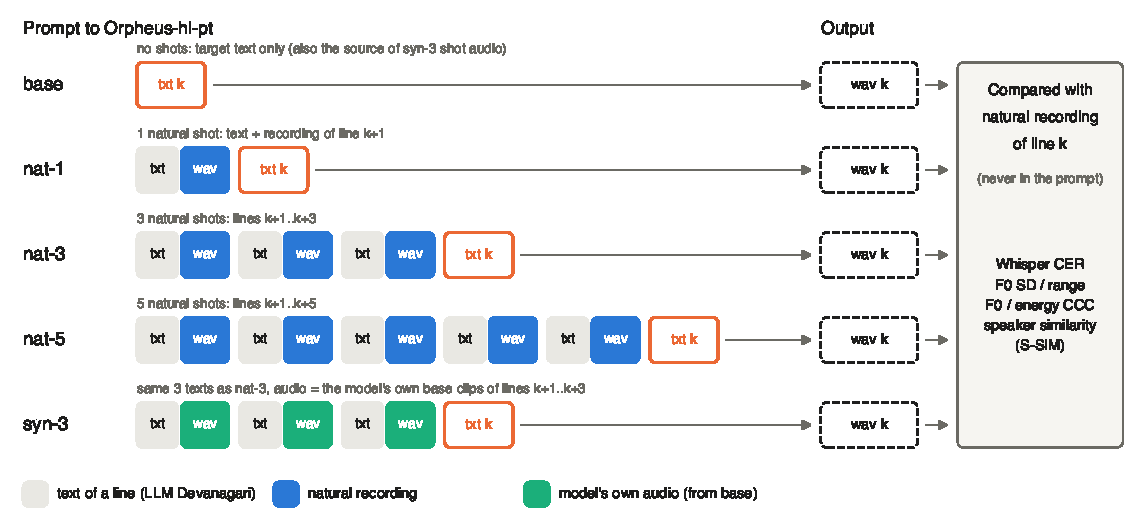
\includegraphics[width=\textwidth]{fig0_setup.pdf}
\caption*{\small\textbf{Figure 1.} Experimental setup. For each speaker, every clip in turn is the target $k$. Shots are the next $n$ clips of the same speaker in a fixed list (folder order of the 100 listening examples). The clips are unrelated lines from different episodes, so this is an arbitrary but fixed choice of other clips, not dialogue context. The target's own recording is never in the prompt. Each prompt ends with the target text, and the model generates its audio. syn-3 uses the same shot texts as nat-3, but with the model's own base clips as shot audio. Every output is compared with the held-out natural recording of line $k$.}\end{figure}

\textbf{Conditions} (150 generated clips, seed 1234, one sample each):

\begin{tabular}{@{}l p{0.8\textwidth}@{}}
\toprule
\textbf{base} & No shots. The model's default delivery, regenerated from the LLM text. \\
\textbf{nat-1/3/5} & 1, 3 or 5 natural recordings of the same speaker, with their text, as shots. The shots for a line are the next $n$ clips of that speaker in a fixed list order (folder order of the 100 listening examples, wrapping around). The clips are unrelated lines from different episodes, so this is an arbitrary, fixed choice of other clips, not preceding dialogue. The line itself is never a shot. \\
\textbf{syn-3} & The same 3 shot texts as nat-3, but with the shot audio taken from \textbf{base}: the model's own synthetic speech (on-policy control). \\
\bottomrule
\end{tabular}

\textbf{Prompt design.} Each shot is a completed text--speech turn; the target text follows as an open turn:
\begin{center}\small\ttfamily
\begin{tabular}{@{}l@{}}
[SOH] maya\_1\_txt [EOT EOH SOA SOS] maya\_1\_wav [EOS EOA]\\
{}[SOH] maya\_2\_txt [EOT EOH SOA SOS] maya\_2\_wav [EOS EOA]\\
{}[SOH] maya\_3\_txt [EOT EOH SOA SOS] maya\_3\_wav [EOS EOA]\\
{}[SOH] maya\_4\_txt [EOT EOH SOA SOS] $\rightarrow$ model generates maya\_4\_wav, stops at [EOS]
\end{tabular}\end{center}
Token ids: SOH 128259, EOT 128009, EOH 128260, SOA 128261, SOS 128257, EOS 128258, EOA 128262. Audio is SNAC 24\,kHz, 7 tokens per frame (no frame deduplication). The target's own recording is never in the prompt; it is used only as the reference. Decoding: temperature 0.6, top-p 0.9, repetition penalty 1.1. Token cap $\approx 2\times$ the expected length of the line (\texttt{token\_budget}). Canopy does not publish the in-context token layout. This layout repeats Orpheus's standard single-turn TTS format once per shot.

\textbf{Metrics.} Whisper-large-v3 CER against the target text. Praat F0 SD and range (semitones), duration, speaking rate and pauses. DTW-aligned F0 and energy correlation (CCC) with the line's natural clip. Speaker similarity (S-SIM): WavLM-SV cosine to the mean embedding of the speaker's \emph{other} 14 natural clips. Paired differences over the 15 lines per speaker, with 95\% bootstrap intervals (2000 resamples).

\section*{Results}
\begin{figure}[H]\centering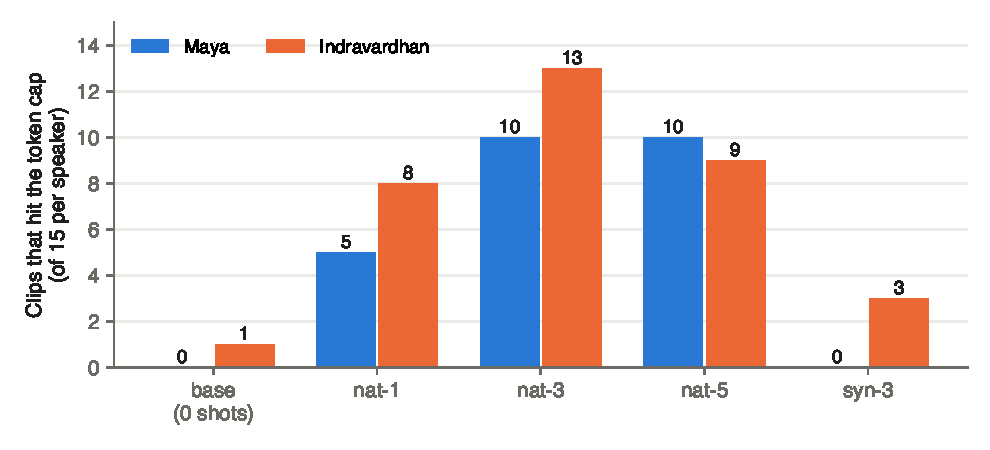
\includegraphics[width=0.78\textwidth]{fig1_runaway.pdf}
\caption*{\small\textbf{Figure 2.} Clips where the model never emitted end-of-speech and was stopped by the token cap. Natural shots trigger it in a third to most of the clips; the model's own shots (syn-3) almost never do.}\end{figure}

\begin{figure}[H]\centering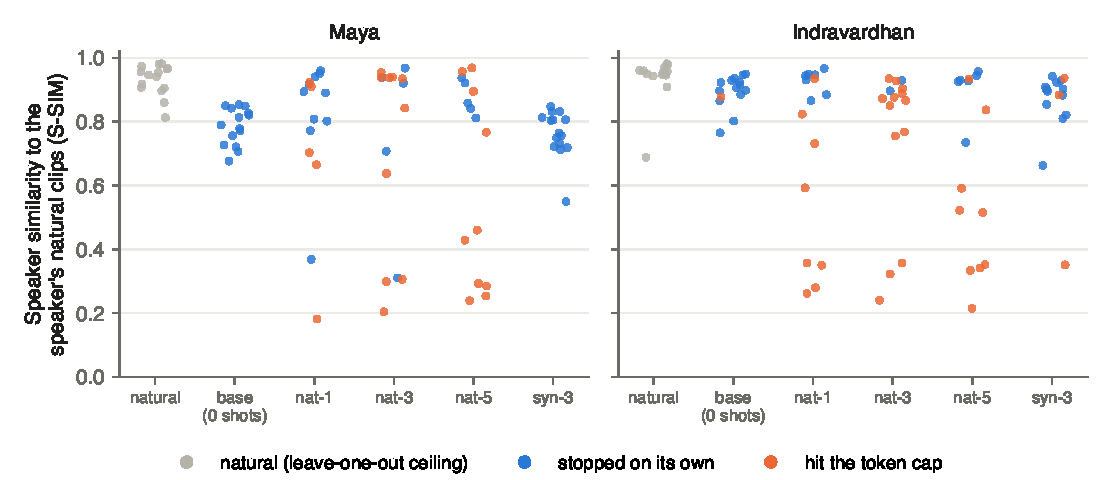
\includegraphics[width=0.88\textwidth]{fig2_ssim.pdf}
\caption*{\small\textbf{Figure 3.} Speaker similarity per clip: cosine similarity between the clip's speaker embedding and the average embedding of the speaker's other 14 natural clips. Embeddings are x-vectors from \href{https://huggingface.co/microsoft/wavlm-base-plus-sv}{WavLM Base+ fine-tuned for speaker verification} (\texttt{microsoft/wavlm-base-plus-sv}; Chen et al., 2022). With natural shots, clips split into two groups: close to the real speaker (as close as the speaker's own recordings), or far off. The far-off ones are almost all runaway clips. The model's default voice is already close to Indravardhan (0.89), so the voice shift is easiest to see for Maya.}\end{figure}

\begin{figure}[H]\centering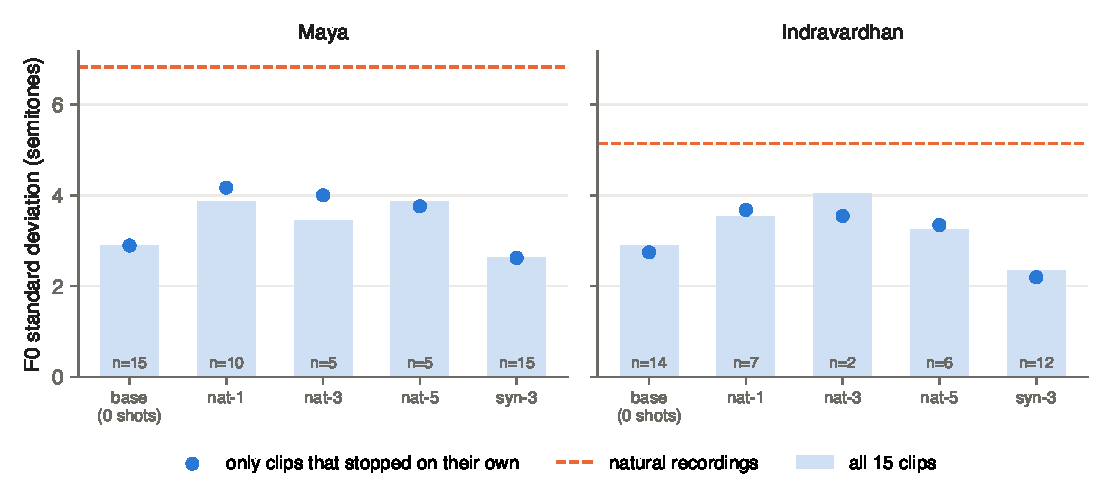
\includegraphics[width=0.88\textwidth]{fig3_f0.pdf}
\caption*{\small\textbf{Figure 4.} Pitch variability. Natural shots raise it, in all clips and in clips that stopped on their own; the model's own shots lower it. All conditions stay well below the natural recordings (dashed line). Few nat-3 clips stopped on their own ($n$ under each bar), so the dots are noisy.}\end{figure}

\begin{figure}[H]\centering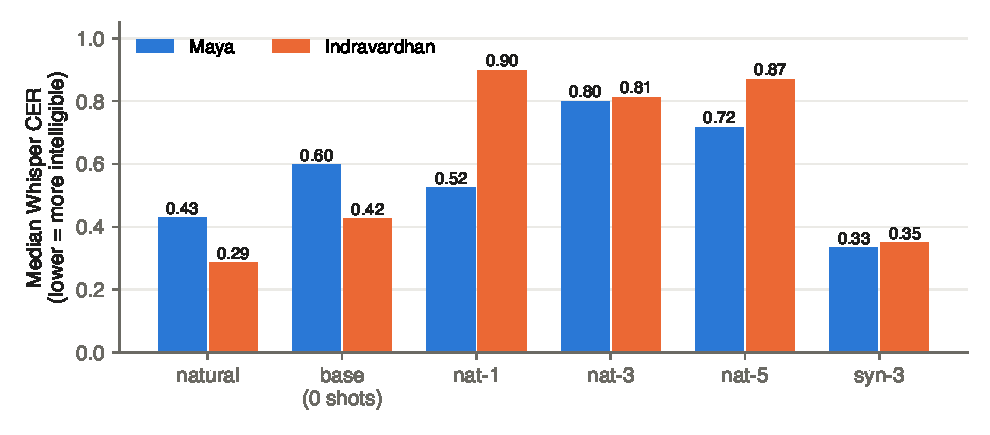
\includegraphics[width=0.78\textwidth]{fig4_cer.pdf}
\caption*{\small\textbf{Figure 5.} Median Whisper CER. Natural shots make the output less intelligible, mostly because of extra audio in the runaway clips. The natural recordings' own CER (0.3--0.4) is the floor for this ASR on this data.}\end{figure}

\section*{What we noticed}
\begin{itemize}
\item \textbf{The runaway clips are long continuations, not repeats of the prompt.} Words from the shot texts appear in the ASR output no more often than in the no-shot control. Some runaway clips have implausible speaking rates for Indravardhan (13--89 words/s), which suggests non-speech audio after the line.
\item \textbf{Why natural shots cause it is untested.} One plausible reason: the sitcom clips do not end in clean silence (laugh track, cut mid-breath), so the examples teach the model that speech does not end cleanly. The model's own shots end the way it expects, and with those it stops normally.
\item \textbf{More shots do not help more.} Speaker match and pitch variability are about the same at 1, 3 and 5 shots; 5 shots is worst on speaker similarity for both speakers.
\item \textbf{Pitch variability rises, but not toward the line's own contour.} The model gets ``livelier'' pitch in general; it does not copy how the real speaker said that particular line (F0 CCC is unchanged). That fits the design: the target line itself is never in the prompt.
\end{itemize}

\section*{Next steps}
\begin{enumerate}
\item \textbf{Listen} to the runaway clips and confirm what the tails are, and to the clean clips for perceived naturalness (bilingual raters).
\item \textbf{Fix the runaway generation before comparing $n$:} trim each natural shot to speech with a short silence at the end, and/or cap generation closer to the line's expected length. Then rerun the same 150 clips.
\item If the rerun is stable, repeat the 1/3/5-shot comparison. Add seeds only if the differences are borderline.
\end{enumerate}

\section*{Appendix}
\subsection*{A.1\quad Per-condition summary (15 lines per speaker)}
\begin{center}\small\begin{tabular}{@{}lrrrrrrrr@{}}
\toprule
\textbf{Condition} & \textbf{Capped} & \textbf{CER} (med.) & \textbf{F0 SD} & \textbf{F0 range} & \textbf{Dur. (s)} & \textbf{F0 CCC} & \textbf{En. CCC} & \textbf{S-SIM}\\
\midrule
\multicolumn{9}{@{}l}{\textbf{Maya}}\\
natural & -- & 0.43 & 6.83 & 21.9 & 5.7 & -- & -- & 0.93\\
base (0 shots) & 0/15 & 0.60 & 2.89 & 9.1 & 6.1 & 0.15 & 0.51 & 0.79\\
nat-1 & 5/15 & 0.52 & 3.86 & 10.7 & 7.8 & 0.16 & 0.51 & 0.78\\
nat-3 & 10/15 & 0.80 & 3.45 & 10.6 & 9.3 & 0.21 & 0.41 & 0.72\\
nat-5 & 10/15 & 0.72 & 3.86 & 11.0 & 10.2 & 0.03 & 0.47 & 0.66\\
syn-3 & 0/15 & 0.33 & 2.62 & 7.8 & 5.6 & 0.05 & 0.57 & 0.76\\
\midrule
\multicolumn{9}{@{}l}{\textbf{Indravardhan}}\\
natural & -- & 0.29 & 5.14 & 16.4 & 5.1 & -- & -- & 0.94\\
base (0 shots) & 1/15 & 0.42 & 2.89 & 8.9 & 7.0 & 0.01 & 0.56 & 0.89\\
nat-1 & 8/15 & 0.90 & 3.54 & 10.8 & 9.9 & -0.10 & 0.46 & 0.72\\
nat-3 & 13/15 & 0.81 & 4.03 & 12.7 & 12.4 & -0.07 & 0.54 & 0.76\\
nat-5 & 9/15 & 0.87 & 3.24 & 8.4 & 10.5 & -0.01 & 0.51 & 0.67\\
syn-3 & 3/15 & 0.35 & 2.35 & 6.4 & 7.1 & 0.10 & 0.63 & 0.84\\
\bottomrule\end{tabular}
\end{center}
Table 1. Means unless noted; F0 in semitones. ``Capped'' = clips stopped by the token cap. Natural S-SIM is leave-one-out (the ceiling). A few clips with too little voicing have no F0 value.

\subsection*{A.2\quad Paired differences, mean [95\% bootstrap CI]}
\begin{center}\scriptsize\setlength{\tabcolsep}{3pt}\begin{tabular}{@{}lllllll@{}}
\toprule
\textbf{Comparison} & \textbf{CER} & \textbf{F0 SD (st)} & \textbf{F0 range (st)} & \textbf{Duration (s)} & \textbf{F0 CCC} & \textbf{S-SIM}\\
\midrule
\multicolumn{7}{@{}l}{\textbf{Maya}}\\
nat-1 $-$ base & -0.02 [-0.13, +0.09] & \textbf{+0.97 [+0.00, +2.09]} & +1.6 [-1.7, +5.4] & +1.7 [-0.1, +3.5] & +0.01 [-0.11, +0.13] & -0.01 [-0.12, +0.09]\\
nat-3 $-$ base & +0.13 [-0.04, +0.31] & +0.55 [-0.77, +1.92] & +1.5 [-2.6, +5.8] & \textbf{+3.2 [+1.5, +4.9]} & +0.04 [-0.10, +0.15] & -0.06 [-0.22, +0.08]\\
nat-5 $-$ base & +0.12 [-0.03, +0.28] & +0.84 [-0.52, +2.38] & +1.5 [-2.6, +6.3] & \textbf{+4.1 [+2.9, +5.3]} & -0.13 [-0.36, +0.08] & \textbf{-0.12 [-0.26, -0.01]}\\
nat-3 $-$ syn-3 & -0.18 [-1.12, +0.36] & +0.83 [-0.26, +1.99] & +2.8 [-0.4, +6.1] & \textbf{+3.7 [+2.1, +5.4]} & +0.16 [-0.06, +0.38] & -0.04 [-0.20, +0.10]\\
nat-3 $-$ nat-1 & +0.15 [-0.02, +0.32] & -0.42 [-2.23, +1.26] & -0.0 [-5.4, +4.8] & +1.5 [-0.8, +3.5] & +0.03 [-0.17, +0.22] & -0.06 [-0.22, +0.09]\\
nat-3 $-$ nat-5 & +0.00 [-0.12, +0.16] & +0.02 [-2.00, +1.80] & +1.0 [-5.4, +6.4] & -0.9 [-2.8, +1.1] & +0.16 [-0.13, +0.41] & +0.06 [-0.14, +0.25]\\
\midrule
\multicolumn{7}{@{}l}{\textbf{Indravardhan}}\\
nat-1 $-$ base & \textbf{+0.43 [+0.04, +1.02]} & +0.62 [-0.71, +2.11] & +1.7 [-2.7, +7.1] & +2.9 [-0.4, +6.0] & -0.12 [-0.24, +0.01] & \textbf{-0.17 [-0.30, -0.05]}\\
nat-3 $-$ base & \textbf{+0.26 [+0.13, +0.39]} & \textbf{+1.19 [+0.06, +2.30]} & +3.9 [-0.1, +8.1] & \textbf{+5.4 [+3.5, +7.4]} & -0.08 [-0.20, +0.05] & \textbf{-0.14 [-0.26, -0.03]}\\
nat-5 $-$ base & \textbf{+0.98 [+0.18, +2.46]} & +0.35 [-0.66, +1.29] & -0.5 [-3.4, +2.1] & \textbf{+3.5 [+1.3, +6.0]} & -0.02 [-0.19, +0.14] & \textbf{-0.22 [-0.36, -0.09]}\\
nat-3 $-$ syn-3 & +0.13 [-0.41, +0.50] & \textbf{+1.76 [+0.63, +2.78]} & \textbf{+6.3 [+3.2, +9.6]} & \textbf{+5.4 [+3.7, +7.1]} & -0.14 [-0.31, +0.02] & -0.08 [-0.21, +0.05]\\
nat-3 $-$ nat-1 & -0.18 [-0.75, +0.21] & +0.35 [-1.01, +1.60] & +0.4 [-4.0, +4.3] & \textbf{+2.5 [+0.9, +4.2]} & +0.04 [-0.12, +0.22] & +0.04 [-0.13, +0.20]\\
nat-3 $-$ nat-5 & -0.72 [-2.27, +0.14] & \textbf{+0.84 [+0.15, +1.51]} & \textbf{+4.6 [+1.5, +7.9]} & \textbf{+1.9 [+0.7, +3.2]} & -0.03 [-0.21, +0.16] & +0.09 [-0.08, +0.26]\\
\bottomrule\end{tabular}
\end{center}
Table 2. B $-$ A over the 15 lines of each speaker; bold = the interval excludes 0. All clips are included, runaway ones too, so these differences mix the prosody effect with the runaway failure.

\subsection*{A.3\quad Data and run}
\begin{itemize}
\item Maya: \texttt{test\_175\_0, train\_1394\_7, val\_131\_1, train\_214\_1, train\_1265\_2, train\_588\_5, train\_376\_7, train\_17\_2, train\_549\_0, train\_240\_3, train\_76\_0, train\_1690\_0, test\_173\_0, train\_723\_2, train\_1241\_0}.
\item Indravardhan: \texttt{train\_1219\_3, train\_1692\_2, test\_158\_0, train\_959\_4, train\_406\_1, train\_1181\_6, train\_291\_0, train\_1472\_2, val\_185\_0, train\_1745\_15, train\_1758\_1, train\_734\_1, train\_1059\_0, train\_1355\_2, train\_378\_4}.
\item Run (kedi): \texttt{/local/speech/users/sp4050/outputs/icl\_pilot/}\allowbreak\texttt{20261112-1324\_maya\_indr30/}, at commit 179d8ba, on one RTX A5500. Generation took 38 min for 21.5 min of audio. Scripts: \texttt{scripts/icl\_generate.py}, \texttt{scripts/icl\_evaluate.py}. Per-clip numbers: \texttt{docs/nshot\_style\_prompting/}\allowbreak\texttt{nshot\_per\_clip.csv}. Plan: \texttt{docs/nshot\_style\_prompting\_plan.md}.
\end{itemize}

\end{document}
